\documentclass[11pt,a4paper]{article}
\usepackage{ifpdf}
\usepackage[utf8]{inputenc}
\usepackage[francais]{babel}
\usepackage[T1]{fontenc}
\usepackage[nottoc, notlof, notlot]{tocbibind}
\usepackage[unicode=true,pdftex,colorlinks=true,linkcolor=black,urlcolor=black,citecolor=black]{hyperref}
\usepackage{natbib}
\usepackage{graphicx}
\usepackage{url}
\usepackage{hyperref}

\parindent 0.8cm
%\setlength{\parskip}{0.5em plus 0.2em minus 0.2em}

\title{Projet Service : ALMA' Turn-keyWeek-End}
\author{Anthony \textsc{Caillaud} Manoël \textsc{Fortun}}
\date{\today}
\ifpdf
\pdfinfo {
/Author (Anthony Caillaud Manoël Fortun)
/Title (Projet Service : ALMA' Turn-keyWeek-End)
/Subject (Projet Service : ALMA' Turn-keyWeek-End)
/Keywords ()
/CreationDate (D:20100329212218)
}
\fi

\begin{document}

\maketitle


\clearpage
\tableofcontents
\clearpage
\section{Introduction}

Dans le cadre du module Service dans lequel nous avons étudié tous les
mécanismes et tous les éléments d'une architecture basée sur les services, nous
avons dû mettre en place une SOA complet. Ce SOA doit permettre à un utilisateur
de réserver plusieurs éléments pour un week-end pour deux personnes. Ces
éléments à réserver sont le voyage jusqu'à la destination, deux tickets pour
une manifestation, une chambre pour une nuit dans un hôtel et un diner dans un
restaurant. Afin d'obtenir une SOA fonctionnelle, nous avons d'abord mis en
place notre base de données et déterminé les tables nécessaires. Ensuite, nous
avons fixé les services nécessaires pour le bon déroulement de l'application, du
choix de l'utilisateur jusqu'aux différentes réservations. Une partie
importante de cette architecture sont les interfaces. L'une
d'entre-elle qui sera la façade de notre application pour l'utilisateur et
l'autre qui sera le back office permettant la gestion des entrées dans les
tables vous seront présentées. Enfin la génération du bon de réservation à
partir des données choisies par l'utilisateur à l'aide d'une transformation
XSLT permettra à celui-ci d'obtenir ce document en dans un fichier pdf.


\section{Définition de la base de données}
Pour cette architecture, nous avons utilisé une base de données comprenant les
différentes tables nécessaires au bon fonctionnement de l'application. Notre
base de données contient donc onze tables.

Tout d'abord, il y cinq tables qui contiennent toutes les entrées représentant
les choix proposés à l'utilisateur. Ces tables sont les suivantes :\\

\begin{itemize}
  \item La table LOCALISATION qui permet de choisir un pays et une ville,
  \item La table TYPE MANIFESTATION qui permet de choisir le type de
  manifestation,
  \item La table MANIFESTATION qui permet de choisir une manifestation d'un
  certain type et qui a lieu dans le pays et la ville choisis,
  \item La table HOTEL qui permet de choisir un hôtel présent dans la ville
  choisie,
  \item La table RESTAURANT qui permet de choisir un restaurant présent dans la
  ville choisie.\\
\end{itemize}
 
Ensuite, cinq autres tables permettent l'enregistrement des différentes
réservations effectuées par l'utilisateur. Ces tables sont les suivantes :\\

\begin{itemize}
  \item La table VOYAGE qui enregistre la réservation du voyage entre la ville
  de départ et la ville d'arrivée,
  \item La table RESERVATION MANIF qui enregistre la réservation des deux tickets
  pour la manifestation choisie,
  \item La table RESERVATION HOTEL qui enregistre la réservation d'une chambre pour
  une nuit dans l'hôtel choisi,
  \item La table RESERVATION RESTAURANT qui enregistre la réservation d'un
  diner au restaurant,
  \item La table RESERVATION qui enregistre toutes les données concernant les
  réservations du week-end.\\
\end{itemize}

Enfin, la dernière table est la table CLIENT qui permet l'enregistrement du nom
et du prénom de l'utilisateur voulant effectuer ce week-end.

\section{Les interfaces}
Pour ce projet, nous avons dû définir deux interfaces. L'une d'entre elle est
une interface Web permettant à un utilisateur de faire des recherches et des
réservations. L'autre, permettra de gérer toutes la base de données définie
précédemment.

\subsection{Définition de l'interface}
\subsubsection{L'interface Web}
Dans cette interface, nous avons gérer les intéractions avec l'utilisateur de
façon dynamique en développement une application Web sous GlassFish ESB. En
effet, au fur et à mesure des choix effectués ou des champs remplis par
celui-ci, l'interface se met à jour.\\


Tout d'abord, cinq champs sont à remplir obligatoirement par l'utilisateur.
Ceux-ci sont son nom, son prénom, la date de la manifestation, le pays et la
ville de départ. 

Une fois ces champs remplis, l'utilisateur doit définir le lieu de la
manifestation. Pour cela, il doit dans un premier temps choisir un pays dans une
liste de pays d'arrivée puis faire un choix dans la liste des villes d'arrivée
correspondantes.

Ensuite, le client devra cliquer sur un bouton permettant d'obtenir les
différents types de manifestations disponibles à cette date et en ce lieu.
Lorsque ce type de manifestation est séléctionné, il peut alors choisir dans des
listes la manifestation à laquelle il veut participer, le restaurant où il veut
dîner et l'hôtel où il veut dormir.\\

Lorsque l'utilisateur a séléctionné les différents éléments nécessaires, il
peut alors en cliquant sur un bouton avoir une géolocalisation de la
manifestation, du restaurant et de l'hôtel grâce à GoogleMaps. La technologie
permettant cet affichage sera décrit dans la partie suivante.

\subsubsection{GoogleMaps}
Pour l'affichage de cette géolocalisation, nous utilisons Google Static Maps
API. Cette API permet d'afficher une image GoogleMaps à l'aide d'une URL fixe
comme par exemple :\\
\begin{verbatim}
http://maps.google.com/maps/api/staticmap?center=Williamsburg,
Brooklyn,NY&zoom=13&size=400x400&markers=color:blue|label
:S|11211|11206|11222&sensor=true_or_false
\end{verbatim}

Ce qui donne à l'affichage :

\begin{figure}[h]
  		\centering
  		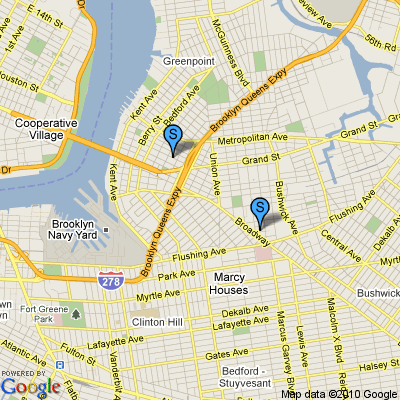
\includegraphics[height=10cm,width=10cm]{staticmap.png}
  		\caption{Exemple de rendu  Google Static Maps API}
  		\label{googlemaps}
\end{figure}

Nous avons donc dû concaténer plusieurs chaînes de caractères comprenant les
données nécessaire à la formation de cette URL. De plus, nous avons défini dans
celle-ci des marqueurs spécifiques afin de bien différencier les adresses de la
manifestation, du restaurant et de l'hôtel.
\clearpage
\subsection{Le back office}

Pour ce projet nous devions aussi développer une application dites de
backoffice. Le rôle d'une application de ce type est de pouvoir administrer
finement toutes les tables de la base de données permettant de voir les
enregistrements existants et d'en insérer de nouveaux.


Nous avions plusieurs pistes pour le développement. Tout d'abord, nous avions
étudié la possibilité de tout générer grâce à Symphony qui permet de générer des
applications backoffice en php. Cependant, nous n'avons pas pu le mettre en
place. Une des raisons supplémentaires est que nous ne savions pas si nous
aurions pu le déployer à la fac. Nous avons donc choisi de développer notre
application en Java classique en Swing comme le suggérait le sujet.



Développer une telle application n'est pas spécialement compliqué lorsqu'on
connait le fonctionnement des technologies nécessaires. Cependant, ce
backoffice ne contient aucun aspects liés au module de service, aucune
technologies vu durant le module n'a été utilisées pour cette partie du projet.


Nous avons donc finalement développer notre application en Swing avec l'aide du
framework Hibernate.



\subsubsection{Architecture}

Avant de nous lancer dans le développement de ce module du projet, nous avons
défini son architecture en fonction des outils utilisés. Le schéma
\ref{backoffice} montre les choix effectués.


\begin{figure}[h]
  		\centering
  		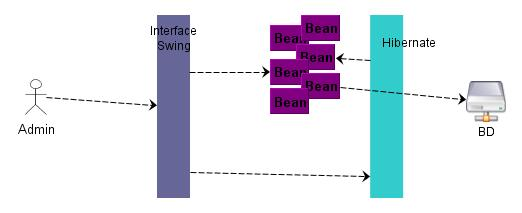
\includegraphics[height=10cm,width=13cm]{backoffice.jpg}
  		\caption{Architecture du backoffice}
  		\label{backoffice}
\end{figure}

Le diagramme \ref{backoffice} montre les interractions basiques entre tous les
éléments où on voit l'utilisateur qui interragit avec l'interface en Swing.
Cette interface interroge la couche hibernate qui gére la liaison
avec la base de donnée et renvoie des classes dites beans représentant les
enregistrements dans la base. Cette architecture et l'utilsation d'Hibernate
nous à permis de gérer la base de données directement en Java sans avoir à
écrire de SQL.


Pour mieux comprendre cette architecture, nous avons jugé nécessaire de fairede
plus amples explications sur Hibernate et la façon dont nous l'avons mis en
oeuvre.


\subsubsection{hibernate}

Hibernate est un framework qui permet un mapping entre objets et base de
données, de manière à ce que les tables et classes soient en relation et que les
enregistrements des tables existent sous la forme d'instances de classes. De
fait, une modification sur une instance est répercutée sur la base de donnée de
façon très simple. Cela permet de facilement faire abstraction de la base et du
langage associé.


Pour mettre en place ce framework dans notre module, nous nous sommes servi de
Netbeans et des fonctions intégrées. Grâce au plugin intégré dans Netbeans nous
avons pu générer de façon automatique les classes représentant les tables, ce qui
nous a fait gagner du temps. Ces classes sont appellés Entity ou beans. La
génération à simplement eut besoin de connaître les identifiants de la BD et sa
localisation, le reste a été automatique. Ensuite, nous avons dû écrire les
quelques méthodes qui permettent de récupérer les objets de la base de données
et faire des actions dessus comme la création, la modification et la
suppresion. Ces fonctions sont contenues dans un objet nommé Session. Nous avons
developpé ces fonctions sans écrire une seule ligne de SQL, le seul code SQL qui
fut écrit le fut pour la création initiale de la base de données.


Une fois l'objet Session défini ainsi que les beans, nous avons utilisé la
bibliothèque Swing pour les afficher et les modifier.

\clearpage
\subsubsection{Swing}

L'utilisation de Swing dans notre application est assez basique, un simple
affichage d'un panel type formulaire pour remplir ou modifier les entités pour
les tables. Ensuite, un objet JTable pour l'affichage de l'ensemble des
enregistrements de la table a été utilisé. Le panel formulaire évolue au fur et à
mesure en changeant la table que l'on souhaite afficher.

Une partie des formulaires de l'application ont été développé grâce au plugin
inclus dans Netbeans. Ce projet a été aussi l'occasion d'utiliser Netbeans en
tant que IDE du début à la fin et pour tous les aspects.

Le but était de faire quelque chose de simple et pratique, sans fioritures
inutile, tout dans la fonctionnalité. C'est pour cela qu'il y a le moins de
fenêtres possibles, pas de menu inutile, le tout très simple.




\section{Les différents services}
Pour notre application, nous avons donc besoin de deux types de services. L'un
qui permet l'intéraction dynamique avec l'utilisateur en fonction de ses
choix. La seconde qui permet le stockage des différentes réservations.
\subsection{Le lien avec l'interface}
Pour ce premier service, nous avons mis en place un module BPEL qui en fonction
des données rentrées par l'utilisateur va aller chercher les informations
nécessaires dans les tables de notre bases de données. 

Par exemple, lorsque l'utilisateur séléctionne un pays, une requête va être
effectuée sur notre table LOCALISATION pour obtenir la liste des villes
correspondantes à ce pays.\\

Dans ce module BPEL, tout consiste donc à tester si les données nécessaires
pour en obtenir une autre sont remplis puis à éxécuter une requête de type FIND
sur les tables.

\subsection{Les réservations}
En ce qui concerne les réservations, nous avons défini d'autre modules BPEL
permettant d'enregistrer dans nos tables les données liées à celles-ci.

Ce service est appelé lorsque l'utilisateur clique sur le bouton ''Valider''
du formulaire.\\ 

Dans les BPEL, on vérifie dans un premier temps si les ID fournis sont valides
puis si il reste encore des places pour la manifestation, le restaurant et
l'hôtel. Si toutes les vérifications sont validées, des requêtes d'insertion
dans les tables sont alors éxécutées.


\section{Génération du bon de réservation}
Une fois toute l'architecture mise en place et les réservations effectuées, il
ne restait plus qu'à produire un bon de réservation dans un fichier au format
PDF.\\

Pour cela, nous avons d'abord produit un fichier XML à partir de toutes les
données récupérées dans le formulaire à l'aide de la librairie JDOM en
Java. 

Ensuite, nous avons utilisé le formateur Apache FOP(Formatting Objects
Processor) qui permet d'obtenir un fichier PDF à l'aide d'un fichier XML et d'un
fichier XSL-FO. Un fichier XSL-FO reste un fichier de transformation XSLT mais
avec des balises "fo" qui permettent d'obtenir la structure d'un fichier PDF.
Une fois le fichier XML créé dans notre code Java, nous l'enregistrons dans un
dossier spécifique où se trouve notre fichier XSL.


Enfin, nous éxécutons la commande nécessaire pour utiliser FOP dans le code Java
pour créer le bon de commande en sortie.




\section{Conclusion}

Ce projet était intéressant du point de vue où il nous permettait de revoir les
différentes technologies vues tout au long du semestre. Cependant, celui-ci
était trop ambitieux par rapport au temps qui nous a été imparti. Nous avons
réussi à produire une application fonctionnelle mais pas sans nuits blanches et
difficultés. Ce projet a été aussi l'occasion pour nous d'utiliser Netbeans en
tant qu'IDE pour le développement de tous les aspects de l'application et cela
convaint de retourner à l'IDE Eclipse. De plus, nous avons rencontré de
nombreux problèmes dû à OpenESB qui nous ont demandé énormément de temps.
Enfin, certains aspects totalement étrangers au module ont pris du temps, comme
le back office ne contenant aucun aspect "service" et le lien avec le service
GoogleMaps.




\end{document}
